
\chapter{Simulations}











\section{Introduction}

Many of the solutions we have covered in this paper require 
numerical techniques for evaluation. We present a different 
approach that serves as both a means of evaluating results, 
and as a way of confirming theories. \bigskip

%For example: \bigskip
%
%\[
%	C_R = \int_{0}^{\infty} \exp \left( -2 \int_{0}^{t} \frac{1 - e^{-u}}{u} du \right) dt
%\]\medskip
%
%which can only be evaluated numerically. 

The Monte Carlo approach is a computational technique that 
is best applied to problems that have a probabilistic 
element. The technique can be summarized as follows: \bigskip

\begin{itemize}
	\item define the range of values to be drawn from
	\item draw values from this range using a distribution
	\item perform a computation on the results 
	\item record the results of the computation
	\item repeat as appropriate
\end{itemize}\medskip

So in the case of the parking problem, the steps would 
be as follows: \bigskip

\begin{itemize}
	\item define the length $L$ on which cars can be parked
	\item draw values from the interval $(0, L)$ using a 
	distribution to simulate the spots taken by cars parking 
	on the length $L$
	\item once no more parking spots remain calculate the 
	coverage, in this case the ratio of cars to the length $L$
	\item record the results of this computation
	\item repeat for as many iterations as required and 
	present statistics of the results of the simulation
\end{itemize}\medskip

The results of the simulation serve as both an estimation 
of a value, but can also be used to confirm that a theory 
is valid where experimental verification might be 
difficult or impractical. \bigskip

We will initially illustrate the usefulness of this approach  
by looking at a simple variation on the parking problem, the 
discrete parking problem (see \cite{krapivsky2010kinetic}), 
where we have an exact result that is easy to evaluate, and 
demonstrate that the technique produces results that are 
consistent with the theory. \bigskip

\newpage






\section{The Discrete Parking Problem}

In the discrete parking problem we have a length $L$ 
made up of discrete sites, and we attempt to park cars 
that occupy two adjacent sites. If a car tries to park 
at two adjacent empty sites, the process is successful, 
otherwise unsuccessful. The process continues until 
there are no more free adjacent empty sites that can 
accommodate cars. \bigskip

The coverage for the discrete parking 
problem is $\theta_{d}(t)$, and the jamming coverage is: \bigskip

\[
	\lim_{t \to \infty} \theta_{d}(t) = 1 - e^{-2}
\]\medskip

which is calculated to be $0.864664$ to six decimal 
places. Below we see the output of a simulation for this problem 
where the number of iterations is set to $10000$ and the 
length $L$ is set to $100000$: \bigskip

%\begin{mdframed}
	\begin{lstlisting}[numbers=none]
    Parking Problem - Discrete Version: results

                                     L:   100000
                            iterations:    10000

                          distribution:
                                  mean: 0.864673
                    standard deviation: 0.000848

	\end{lstlisting} \bigskip
%\end{mdframed} \bigskip

In figure \ref{fig:ps1} we see a plot of the distribution 
of results from our simulation. It has the familiar bell 
curve shape which would imply the simulation produces 
results that are normal, or nearly normal, which in turn 
tells us, for example, that $95\%$ of the results are 
within $2$ standard deviations of the mean. This in itself 
should give us confidence in the technique. \bigskip

\begin{figure}[h!]
	\centering
	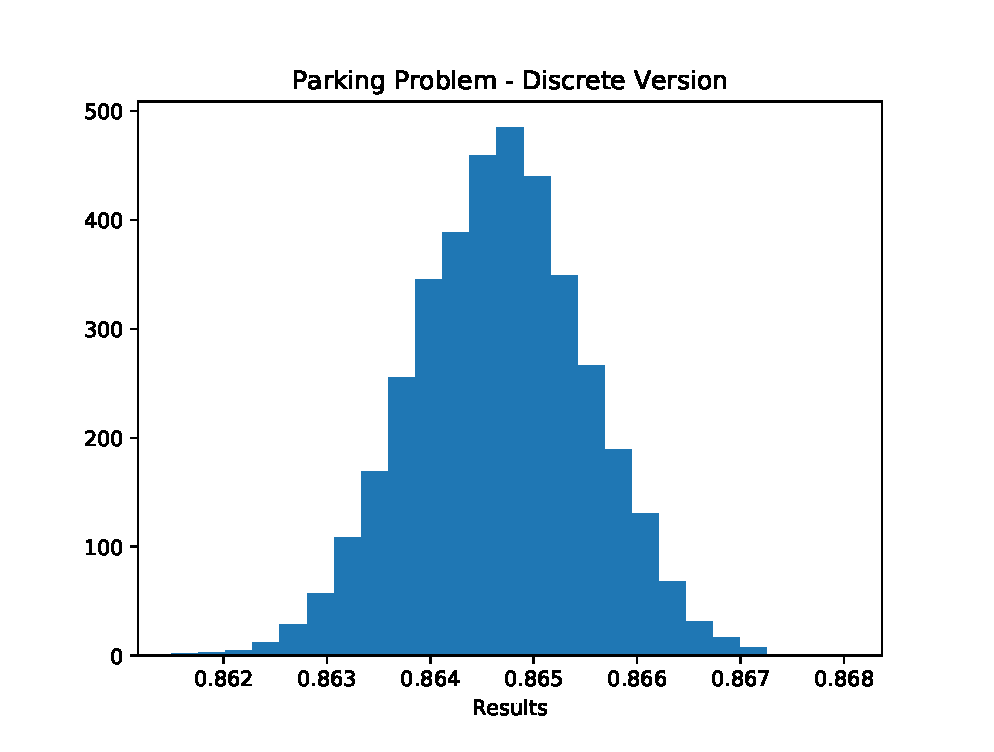
\includegraphics[scale = 0.65]{parking_simulation_01.eps}
%	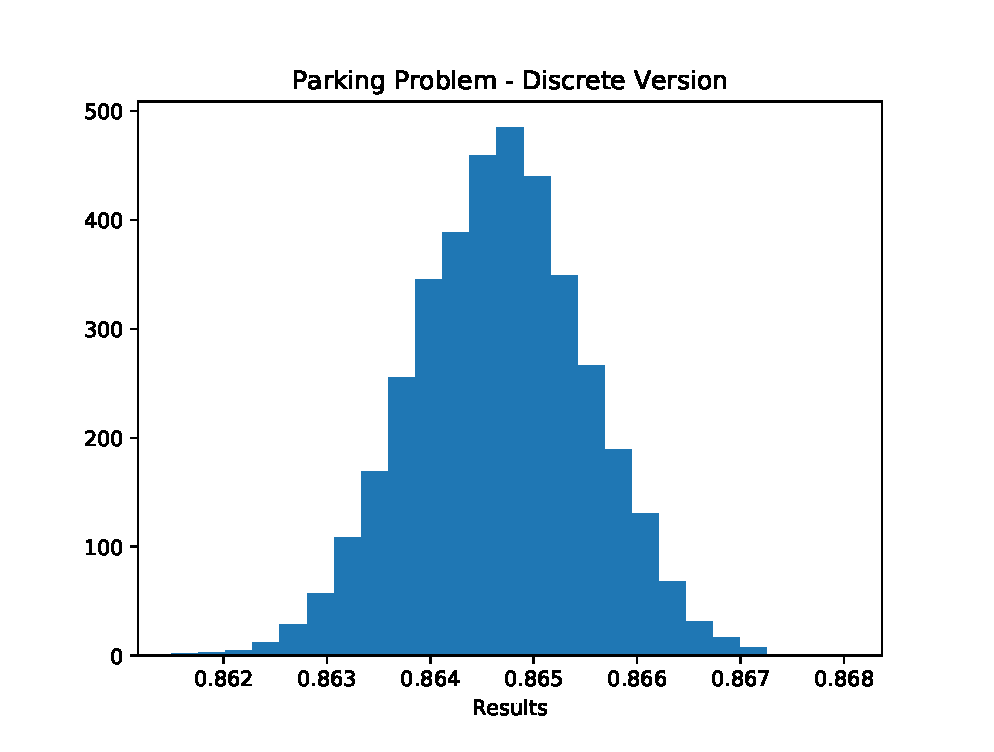
\includegraphics[width=\textwidth]{parking_simulation_01.eps}
	\caption{Histogram of the parking problem simulation - discrete case}
	\label{fig:ps1}
\end{figure}\medskip

So with not much effort we seem to have arrived at an 
alternative approach to numerical techniques for 
evaluation of sometimes complicated results. We see 
consistency between the result calculated above, and 
from our simulation, which would seem to validate the 
mathematics. \bigskip

%\newpage








\section{The Parking Problem}

Next we will simulate the parking problem. We construct 
the simulation similarly to the discrete case, except 
in this case we do not park in discrete adjacent places, 
so our implementation is actually simpler. The jamming 
coverage for the parking problem is: \bigskip

\[
	C_R = \int_{0}^{\infty} \exp \left( -2 \int_{0}^{t} \frac{1 - e^{-u}}{u} du \right) dt
\]\medskip

which can only be evaluated numerically, and is 
calculated to be $0.747598$ to six decimal places. We 
see below the output of a simulation for this problem 
with the number of iterations set to $10000$ and $L$ 
set to $100000$: \bigskip

%\begin{mdframed}
	\begin{lstlisting}[numbers=none]
                    Parking Problem: results

                                  L:   100000
                         iterations:    10000

                       distribution:
                               mean: 0.747602
                 standard deviation: 0.000617

	\end{lstlisting} \bigskip
%\end{mdframed} \bigskip

In figure \ref{fig:ps2} we see a plot of the distribution 
of results from our simulation. Once again, we see the 
familiar bell curve shape which would again imply the 
simulation produces results that are normal, or nearly 
normal. \bigskip

\begin{figure}[h!]
	\centering
	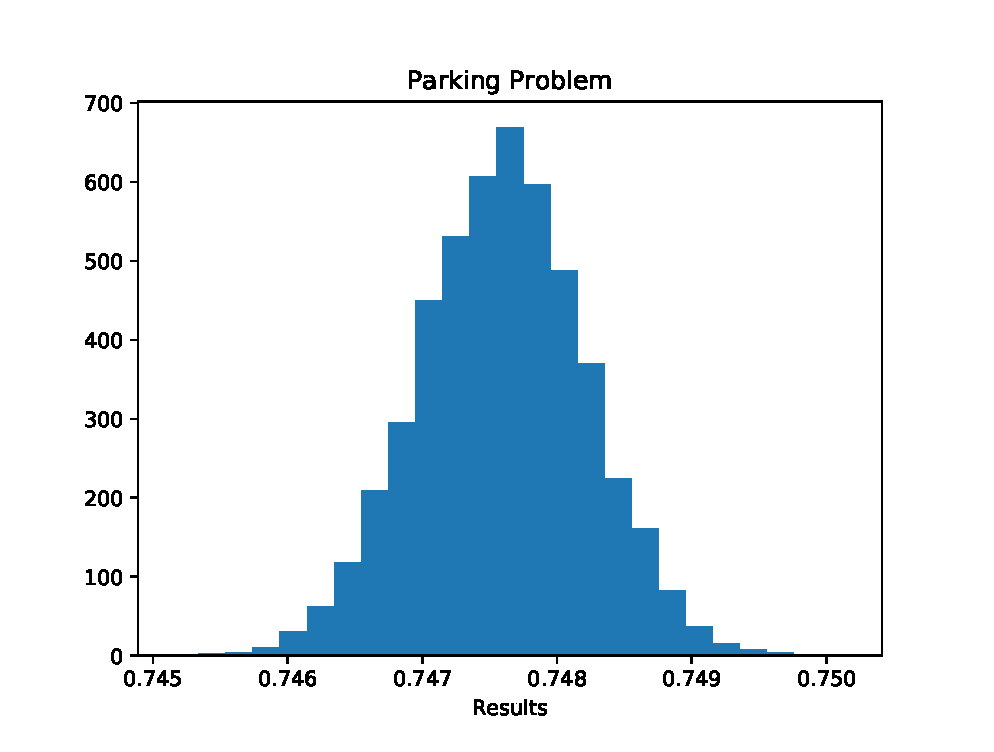
\includegraphics[scale = 0.65]{parking_simulation_02.eps}
%	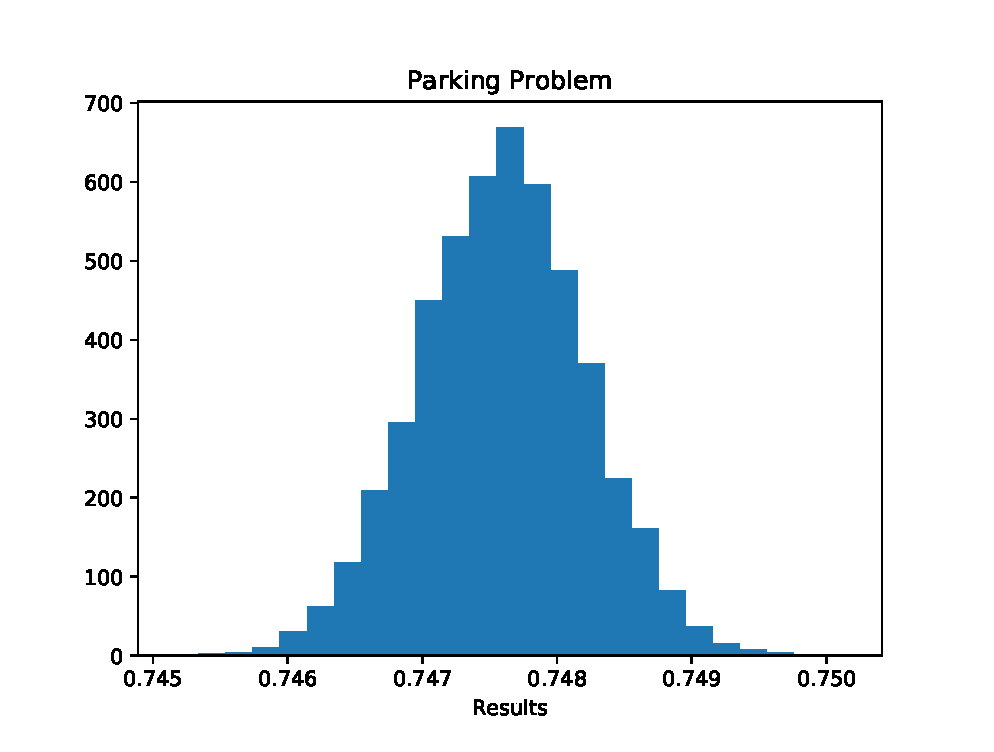
\includegraphics[width=\textwidth]{parking_simulation_02.eps}
	\caption{Histogram of the parking problem simulation}
	\label{fig:ps2}
\end{figure}\medskip

Once again we see clear consistency between the numerically 
evaluated result, and the result of the simulation. So again 
we have provided a pretty successful means of evaluating our 
constant other than the standard numerical approach. \bigskip

%\newpage







\section{Parking with overlap}

Next we will simulate parking with overlap. We construct 
the simulation similarly to the earlier cases, except 
in this case we park by exclusion zone. The coverage by 
cars for parking with overlap is: \bigskip

\begin{eqnarray*}
	\Theta_{\phi}(t) = 
	\begin{dcases}
		(1 - 2 \phi) \int_{0}^{t} F_{\phi}(\tau) d \tau  + \int_{0}^{t} F_{\phi}(\tau) \frac{2}{\tau} (1 - e^{-\phi \tau}) d \tau			& \text{for } \phi < \frac{1}{2} \\\\
		1 - F_{\phi}(t) e^{(1 - 2 \phi)t}																									& \text{for } \phi \geq \frac{1}{2} 
	\end{dcases}
\end{eqnarray*}\medskip

The jamming coverage for a selection of values for $\phi$ 
as $t \to \infty$ is shown below in table \ref{table:2}: \bigskip

\begin{table}[h!]
	\centering
	\begin{tabular}{|l | l|} 
		\hline
		$\phi$ & $\lim_{t \to \infty} \Theta_{\phi}(t)$ \\ [1ex] 
		\hline
		0.1 & 0.816909 \\ 
		0.2 & 0.880028 \\ 
		0.3 & 0.936238 \\ 
		0.4 & 0.980342 \\ 
		0.5 & 1 \\ 
		\hline
	\end{tabular}
	\caption{$\lim_{t \to \infty} \Theta_{\phi}(t)$}
	\label{table:2}
\end{table}\medskip

As we see, the coverage gets closer to full coverage (i.e. $1$) 
as $\phi \to 0.5$. \bigskip

\newpage

We see below the output of a simulation for this problem with 
the number of iterations set to $10000$, $L$ set to $100000$, 
and with $\phi$ set to $0.1$: \bigskip

%\begin{mdframed}
	\begin{lstlisting}[numbers=none]
    Parking Problem - Overlap Version: results

                                    L:   100000
                              overlap:      0.1
                           iterations:    10000

                         distribution:
                                 mean: 0.816894
                   standard deviation: 0.000584

	\end{lstlisting} \bigskip
%\end{mdframed} \bigskip

In figure \ref{fig:ps3} we see a plot of the distribution 
of results from our simulation for $\phi = 0.1$: \bigskip

\begin{figure}[h!]
	\centering
	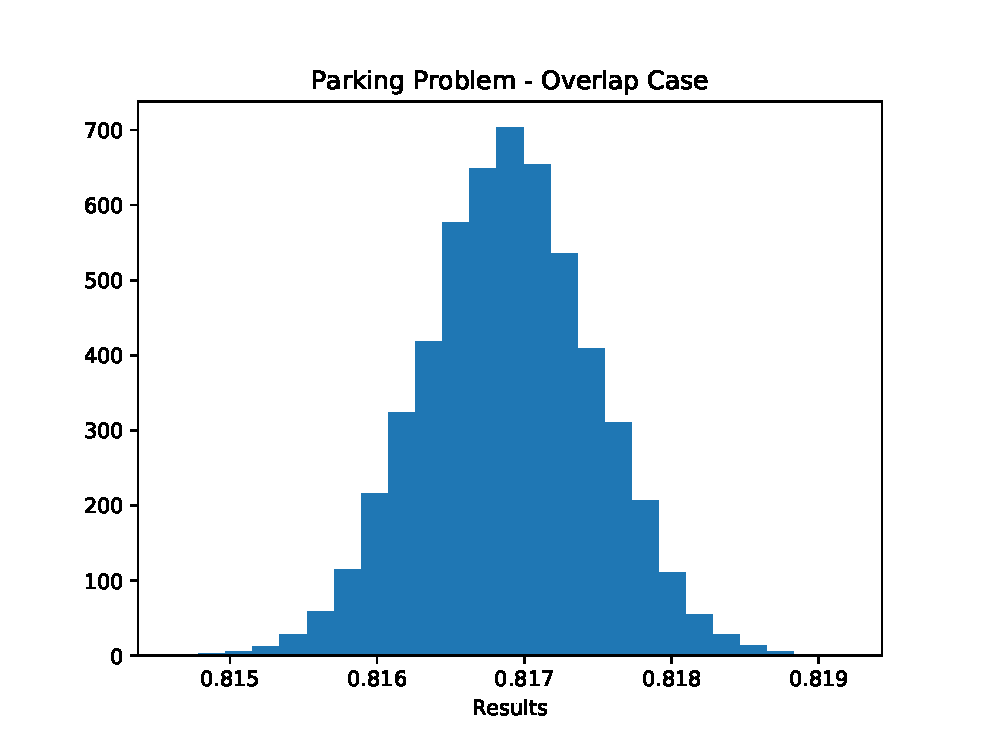
\includegraphics[scale = 0.65]{parking_simulation_03.eps}
	%	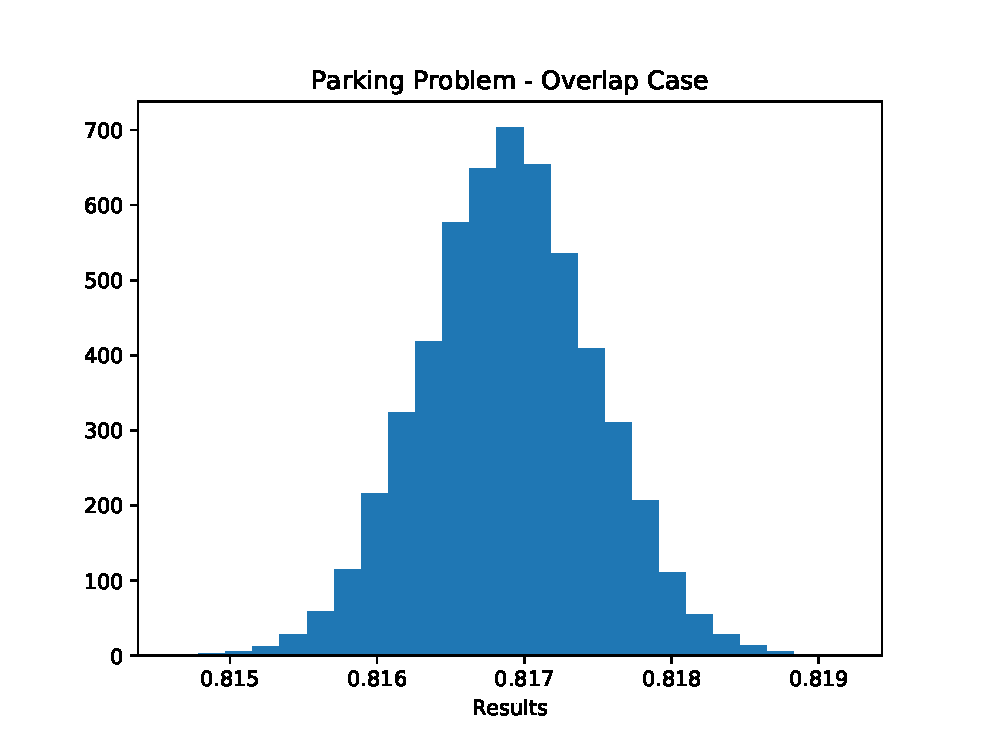
\includegraphics[width=\textwidth]{parking_simulation_03.eps}
	\caption{Histogram of the parking with overlap simulation - $\phi = 0.1$}
	\label{fig:ps3}
\end{figure}\medskip

\newpage

We see below the output of a simulation for this 
problem with the number of iterations set to $10000$, 
$L$ set to $100000$, and with $\phi$ set to $0.2$: \bigskip

%\begin{mdframed}
	\begin{lstlisting}[numbers=none]
    Parking Problem - Overlap Version: results
	
                                    L:   100000
                              overlap:      0.2
                           iterations:    10000
	
                         distribution:
                                 mean: 0.880027
                   standard deviation: 0.000477

	\end{lstlisting} \bigskip
%\end{mdframed} \bigskip

In figure \ref{fig:ps4} we see a plot of the distribution 
of results from our simulation for $\phi = 0.2$: \bigskip

\begin{figure}[h!]
	\centering
	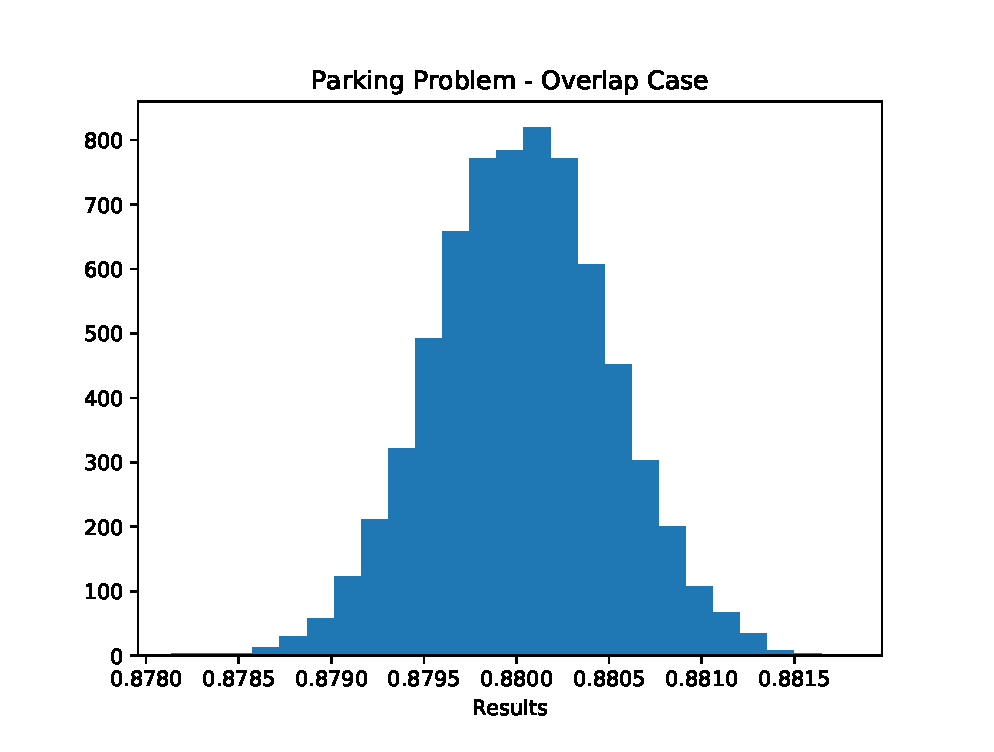
\includegraphics[scale = 0.65]{parking_simulation_04.eps}
	%	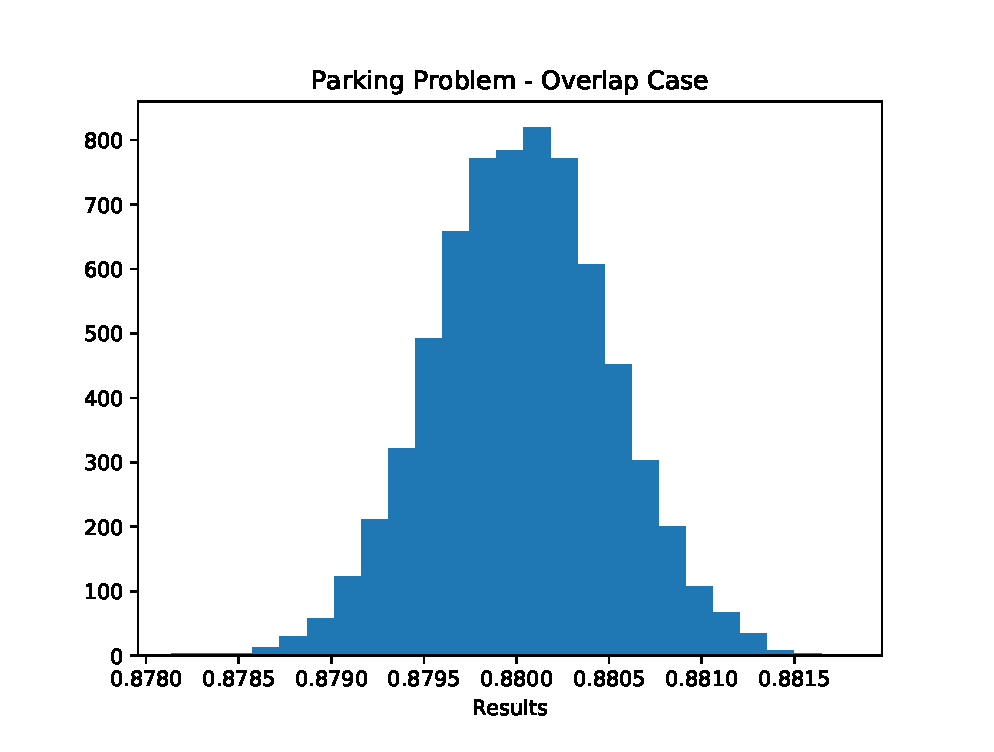
\includegraphics[width=\textwidth]{parking_simulation_04.eps}
	\caption{Histogram of the parking with overlap simulation - $\phi = 0.2$}
	\label{fig:ps4}
\end{figure}\medskip

\newpage

We see below the output of a simulation for this 
problem with the number of iterations set to $10000$, 
$L$ set to $100000$, and with $\phi$ set to $0.3$: \bigskip

%\begin{mdframed}
	\begin{lstlisting}[numbers=none]
    Parking Problem - Overlap Version: results

                                    L:   100000
                              overlap:      0.3
                           iterations:    10000

                         distribution:
                                 mean: 0.936235
                   standard deviation: 0.000327

	\end{lstlisting} \bigskip
%\end{mdframed} \bigskip

In figure \ref{fig:ps5} we see a plot of the distribution 
of results from our simulation for $\phi = 0.3$: \bigskip

\begin{figure}[h!]
	\centering
	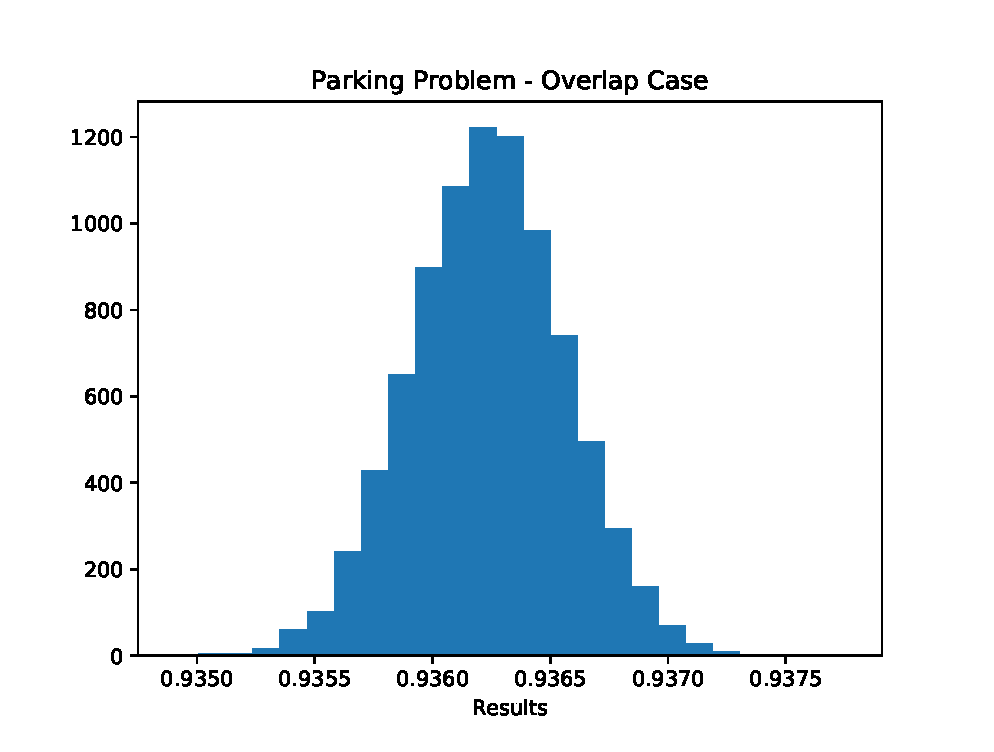
\includegraphics[scale = 0.65]{parking_simulation_05.eps}
	%	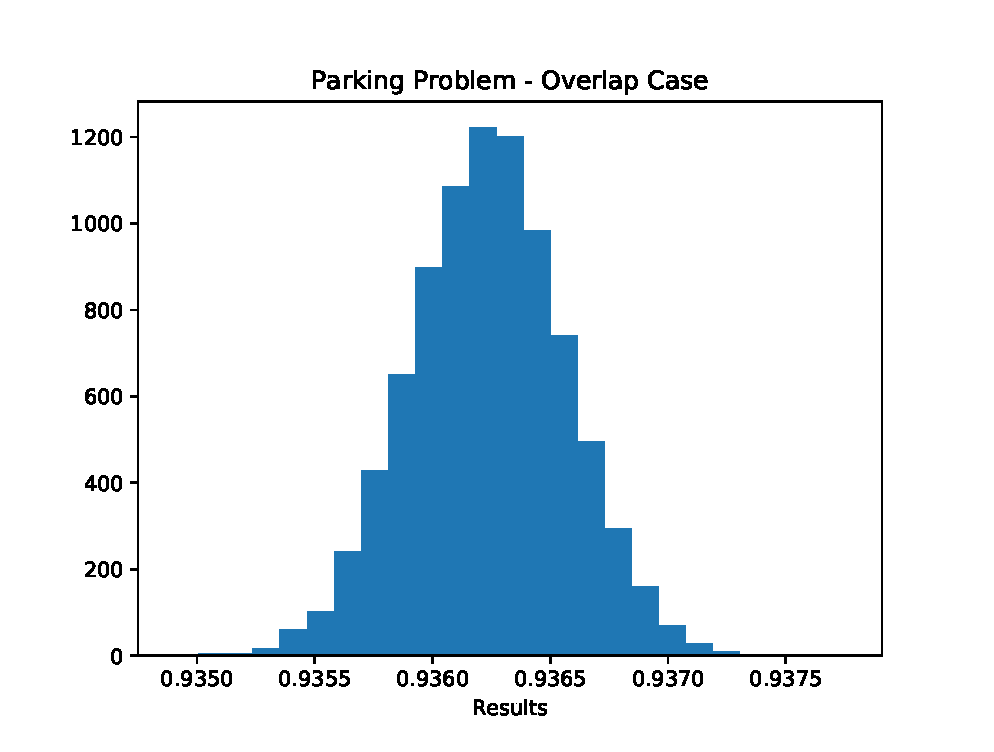
\includegraphics[width=\textwidth]{parking_simulation_05.eps}
	\caption{Histogram of the parking with overlap simulation - $\phi = 0.3$}
	\label{fig:ps5}
\end{figure}\medskip

\newpage

We see below the output of a simulation for this 
problem with the number of iterations set to $10000$, 
$L$ set to $100000$, and with $\phi$ set to $0.4$: \bigskip

%\begin{mdframed}
	\begin{lstlisting}[numbers=none]
    Parking Problem - Overlap Version: results

                                    L:   100000
                              overlap:      0.4
                           iterations:    10000

                         distribution:
                                 mean: 0.980344
                   standard deviation: 0.000144

	\end{lstlisting} \bigskip
%\end{mdframed} \bigskip

In figure \ref{fig:ps6} we see a plot of the distribution 
of results from our simulation for $\phi = 0.4$: \bigskip

\begin{figure}[h!]
	\centering
	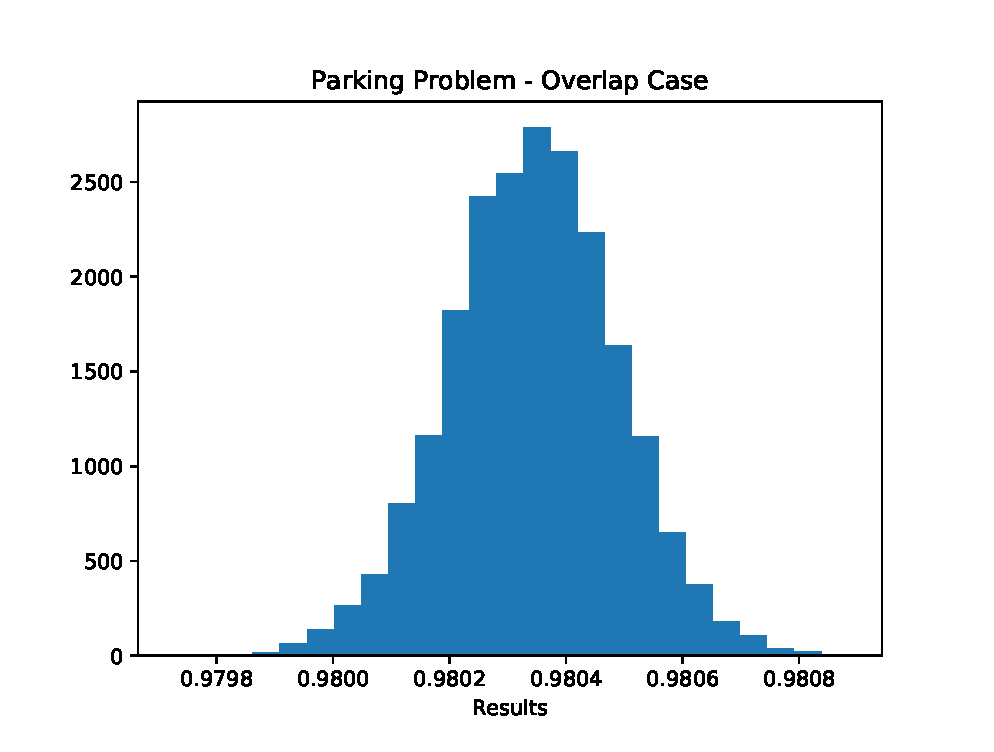
\includegraphics[scale = 0.65]{parking_simulation_06.eps}
	%	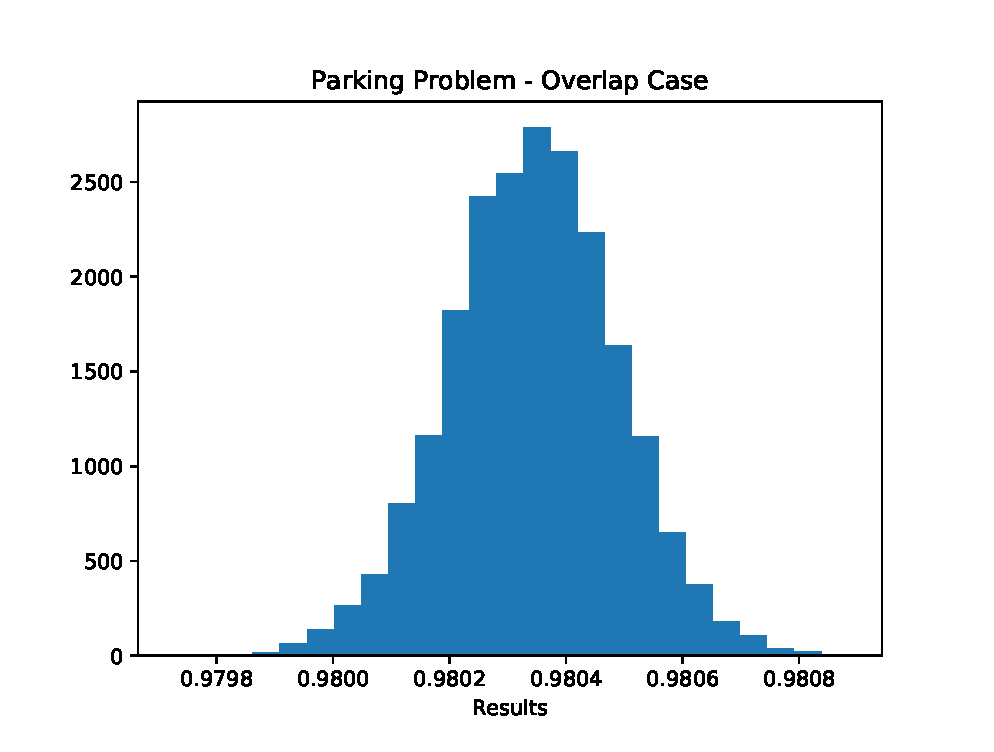
\includegraphics[width=\textwidth]{parking_simulation_06.eps}
	\caption{Histogram of the parking with overlap simulation - $\phi = 0.4$}
	\label{fig:ps6}
\end{figure}\medskip

\newpage

We see below the output of a simulation for this 
problem with the number of iterations set to $10000$, 
$L$ set to $100000$, and with $\phi$ set to $0.5$: \bigskip

%\begin{mdframed}
	\begin{lstlisting}[numbers=none]
    Parking Problem - Overlap Version: results

                                    L:   100000
                              overlap:      0.5
                           iterations:    10000

                         distribution:
                                 mean: 1.000000
                   standard deviation: 0.000000

	\end{lstlisting} \bigskip
%\end{mdframed} \bigskip

In figure \ref{fig:ps7} we see a plot of the distribution 
of results from our simulation for $\phi = 0.5$: \bigskip

\begin{figure}[h!]
	\centering
	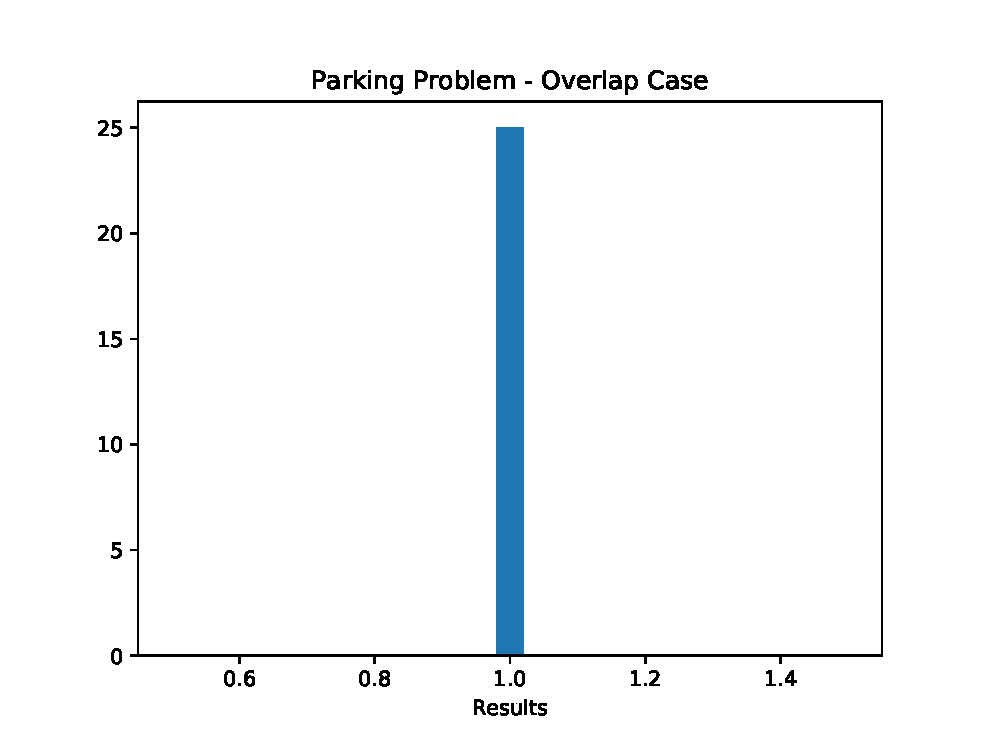
\includegraphics[scale = 0.65]{parking_simulation_07.eps}
%	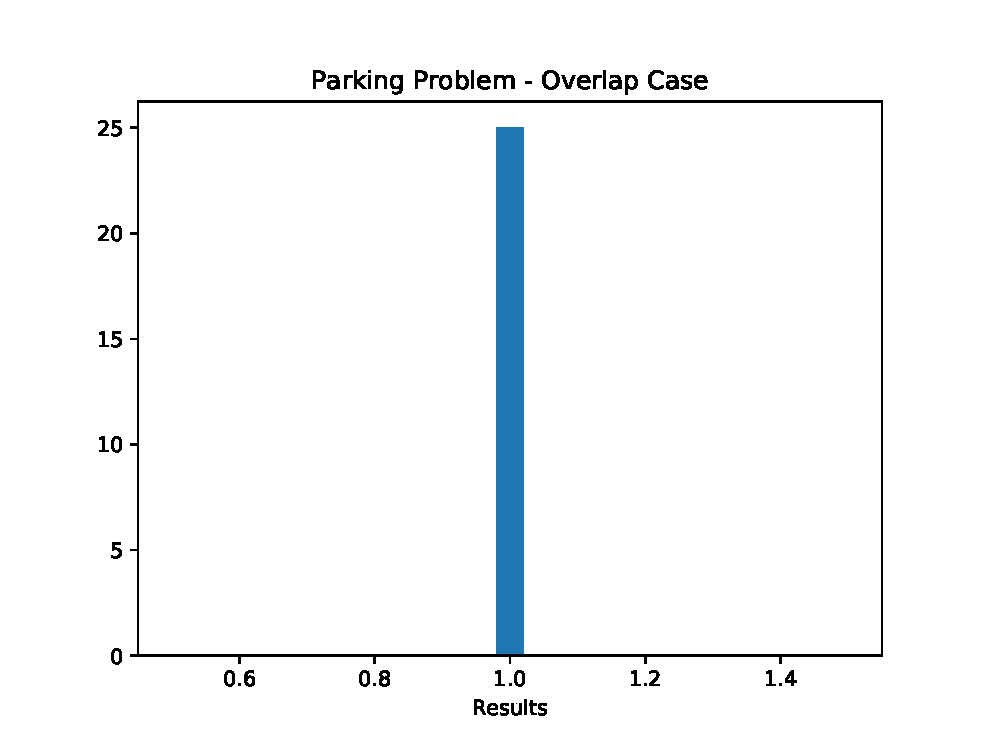
\includegraphics[width=\textwidth]{parking_simulation_07.eps}
	\caption{Histogram of the parking with overlap simulation - $\phi = 0.5$}
	\label{fig:ps7}
\end{figure}\medskip

\newpage

So again we see strong consistency between the results 
of our simulations, and the corresponding calculated results. 
And the consistent results serve to verify our approach. \bigskip















\section{Remarks}

There are two approaches to implementing simulations: \bigskip

\begin{itemize}
	\item an iterative approach - ordinarily more faithful to the problem, 
	but can take a long time to complete
	\item a recursive approach - more suited to evaluating results, and 
	completes relatively quickly
\end{itemize}\medskip

In the context of our simulations, if we want to confirm that we have 
modelled the process correctly, we might choose an iterative implementation, 
in which case the outcome will be more accurate the more iterations we 
perform, and for larger values of $L$, but if the number of iterations is 
too great, and if $L$ is too large, then the simulation may take a very long 
time to complete. \bigskip

So there needs to be a trade-of made: \bigskip

\begin{itemize}
	\item if high accuracy of the outcome is required, then you should 
	use lots of iterations, and set $L$ to be as large as possible
	\item if confirmation of a theory is all that is required, then 
	fewer iterations will be necessary, and a shorter $L$ will suffice
	\item if the calculation of a value is required, then the recursive 
	approach should be used
\end{itemize}\medskip










